\chapter{Wave Propagation}
\label{chapter:introduction}

Before talking about antennas,
we must first understand some things about how a wave propagates in space.

\section{Huygens principle}
\begin{wrapfigure}{r}{0.35\textwidth}
	\centering
	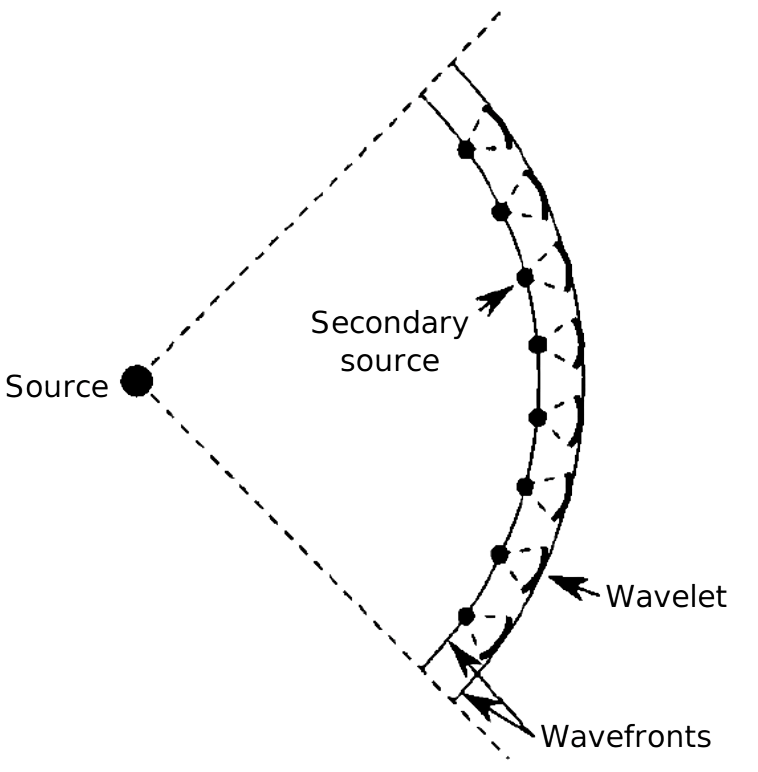
\includegraphics[width=0.35\textwidth]{figures/1.png}
	\caption{}
	\label{1}
	\vspace{1cm}
	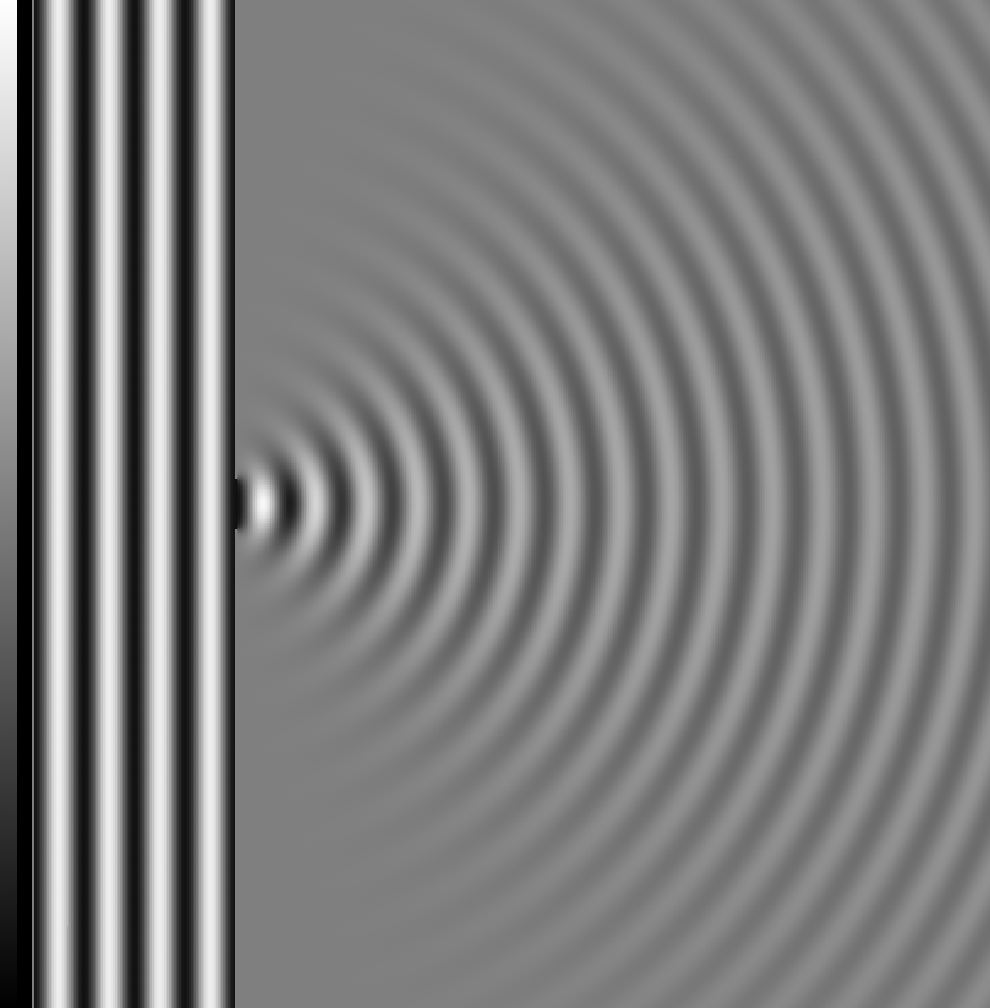
\includegraphics[width=0.35\textwidth]{figures/wave-diffraction}
	\caption{}
	\label{2}
\end{wrapfigure}

Huygens' principle states that every point on a wave can be considered as a source of a wave.

As clearly shown in [Figure \ref{1}], after the wave spreads from the main source, each point on the wave acts as a source of waves. However, since the points composing the wave are theoretically infinite, the sum of the waves generated by all these points results in a smooth wave without distortions.

\section{Wave diffraction}
Therefore, when a wave hits a barrier, part of the wave (part of the wave sources) passes through, and a phenomenon called wave diffraction [Figure \ref{2}] occurs.

When the wave passes through a very small slit, a wave is produced on the other side of the barrier in the shape of a semicircle (or a hemisphere if we look at it from a three-dimensional perspective).

\section{Double slit experiment}
This is one of the most famous experiments in modern physics and quantum mechanics. However, we will discuss the experiment from a wave perspective only.

When a wave passes through two slits, each slit allows a small portion of the wave to pass through. This portion behaves as a single-point wave source, creating a semicircular wave.

The two waves intersect, creating areas where in phase regions intersect, increasing the wave's amplitude (constructive interference). 
Conversely, out-of-phase regions intersect, decreasing the wave's amplitude (destructive fading), as we can see Figure[\ref{fig:double-slit}], the amplitude of the beam in the middle is the most saturated one, and we loss saturation gradually surrounding beams as we go further away.

\newpage
\begin{figure}[!h]
	\centering
	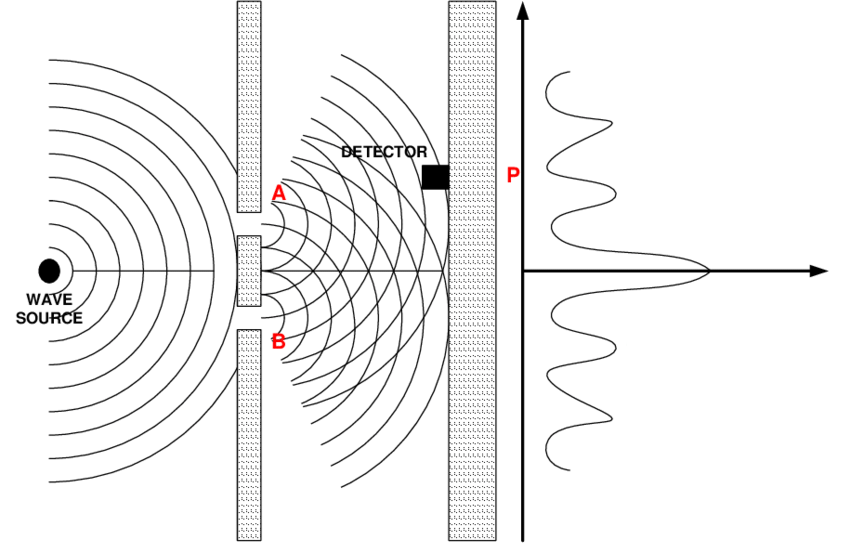
\includegraphics[width=0.7\linewidth]{figures/Double-slit-experiment-illustrating-the-wave-behavior-of-light}
	\caption{}
	\label{fig:double-slit}
\end{figure}

\section{antenna array}
In the previous experiment, we used only two wave sources in a three-dimensional space.

In a commercial antenna array, we use more than two wave sources (antennas) arranged on a three-dimensional surface. In this case, we get a set of beams, as happened in the double-slit experiment. However, as the number of antennas in the array increases, the concentration of the beam in the center (main lobe) increases at the expense of the side beams (side lodes).

This makes the wave emitted by the antenna somewhat similar to a laser. Figure[\ref{fig:1532895074001}].

the beam in the middle has much more SNR than a single antenna with the same power of the system will have in the same distance.
so we use this phenomenon to decrease the probability of error of the system so we can decrease the BER.

\begin{figure}[!h]
	\centering
	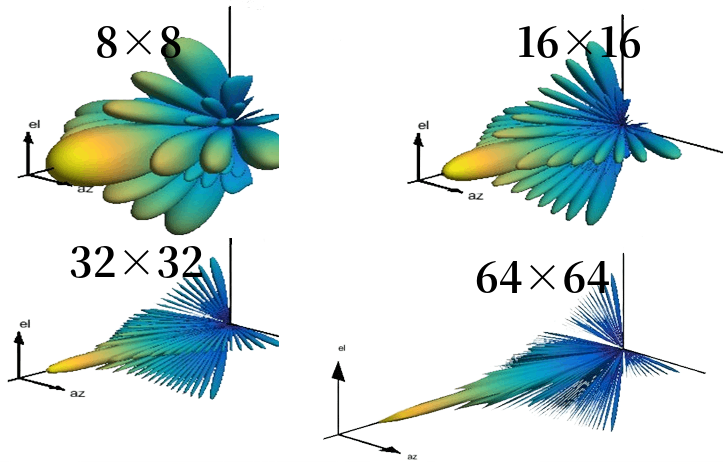
\includegraphics[width=0.6\linewidth]{figures/beams}
	\caption{}
	\label{fig:1532895074001}
\end{figure}

\newpage
\section{Spatial Diversity}
it's the process of staking more then one array it the \Tx (MISO) or the \Rx (SIMO) or both of them (MIMO) to decrease the probability of error of the communication system and to concentrate the wave into a beam in a directed angle.


Figure[\ref{fig:spatial-diversity}].
\begin{figure}[!h]
	\centering
	\includegraphics[width=1\linewidth]{"figures/Spatial Diversity"}
	\caption{Spatial Diversity}
	\label{fig:spatial-diversity}
\end{figure}